\section{Methodology}
This section will introduce the main work of this paper.
In Section~\ref{subsec:RAGSVAG}, it introduces the proposed customized RAG framework for NL2SVA.
In Section~\ref{subsec:synthetic-finetuning-dataset}, it introduces the proposed fine-tuning dataset with prompt-guided explanations.
In Section~\ref{subsec:Evaluation-Dataset}, it introduces the proposed evaluation dataset.

\subsection{Customized RAG Framework for NL2SVA}
\label{subsec:RAGSVAG}
The overall flow is illustrated in Fig.~\ref{fig:overallflow-RAGSVAG}. 
% Starting from a given Verilog design and its corresponding assertion specification, the framework first utilizes a customized RAG pipeline to retrieve relevant contextual information with the input assertion specification. 
Given a Verilog design and a natural language assertion specification, the framework first applies a customized RAG to retrieve relevant contextual information based on the input specification.
The customized RAG component is built upon two key techniques: 
\textit{dynamic splitting} for constructing a code-based retrieval database from SystemVerilog textbooks (Section~\ref{subsubsec:Dynamic-Splitting}), and \textit{HybridRetrieval} that enhances the retrieval  by integrating global semantic retrieval with keyword-guided retrieval (Section~\ref{subsubsec:HybridRetrieval}). 
The retrieved information is incorporated into the \textit{Initial Input Prompt} to assist in generating a better initial SVA. 
The initial input prompt is shown in Fig.~\ref{fig:initial_sva_generation_prompt}.
\begin{figure}
    \centering
    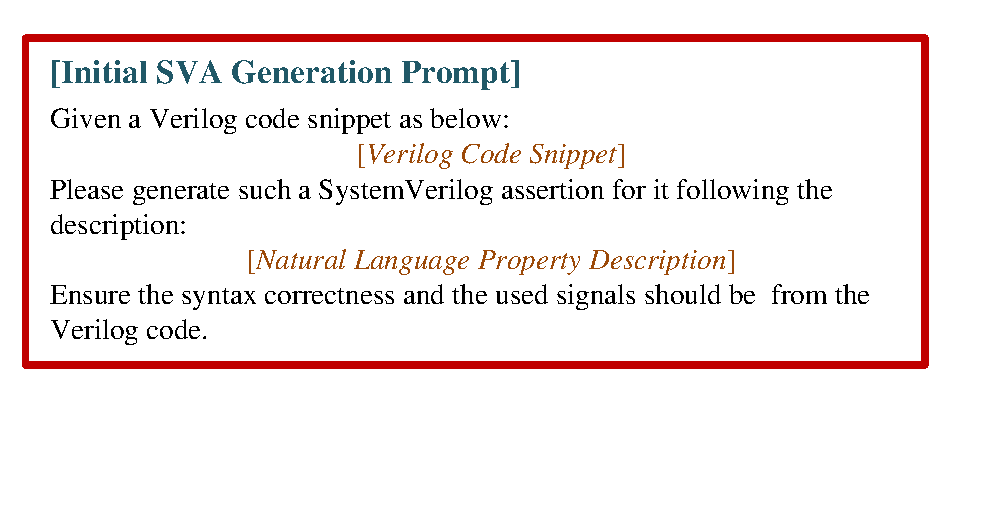
\includegraphics[width=\linewidth]{Figs/Initial-SVA-Generation.pdf}
    \caption{Initial SVA generation prompt.}
    \label{fig:initial_sva_generation_prompt}
\end{figure}
% \begin{framed}
% \begin{verbatim}
% // Initial SVA Generation Prompt
% Given a Verilog code snippet as below:
% ......

% Please generate such a systemverilog 
% assertion for it following the 
% description:
% ......

% Ensure the syntax correctness and the 
% used signals should be from the 
% verilog code.
% \end{verbatim}
% \end{framed}

To improve correctness of the generated assertion, an \textit{SVA operator-based rechecking} is applied (Section~\ref{subsubsec:SVA-Op-based-Rechecking}). 
This refinement step verifies and corrects the usage of SVA operators, ensuring better alignment between the generated assertion and the intended property description. 
Finally, it outputs a refined assertion.

\begin{figure}
    \centering
    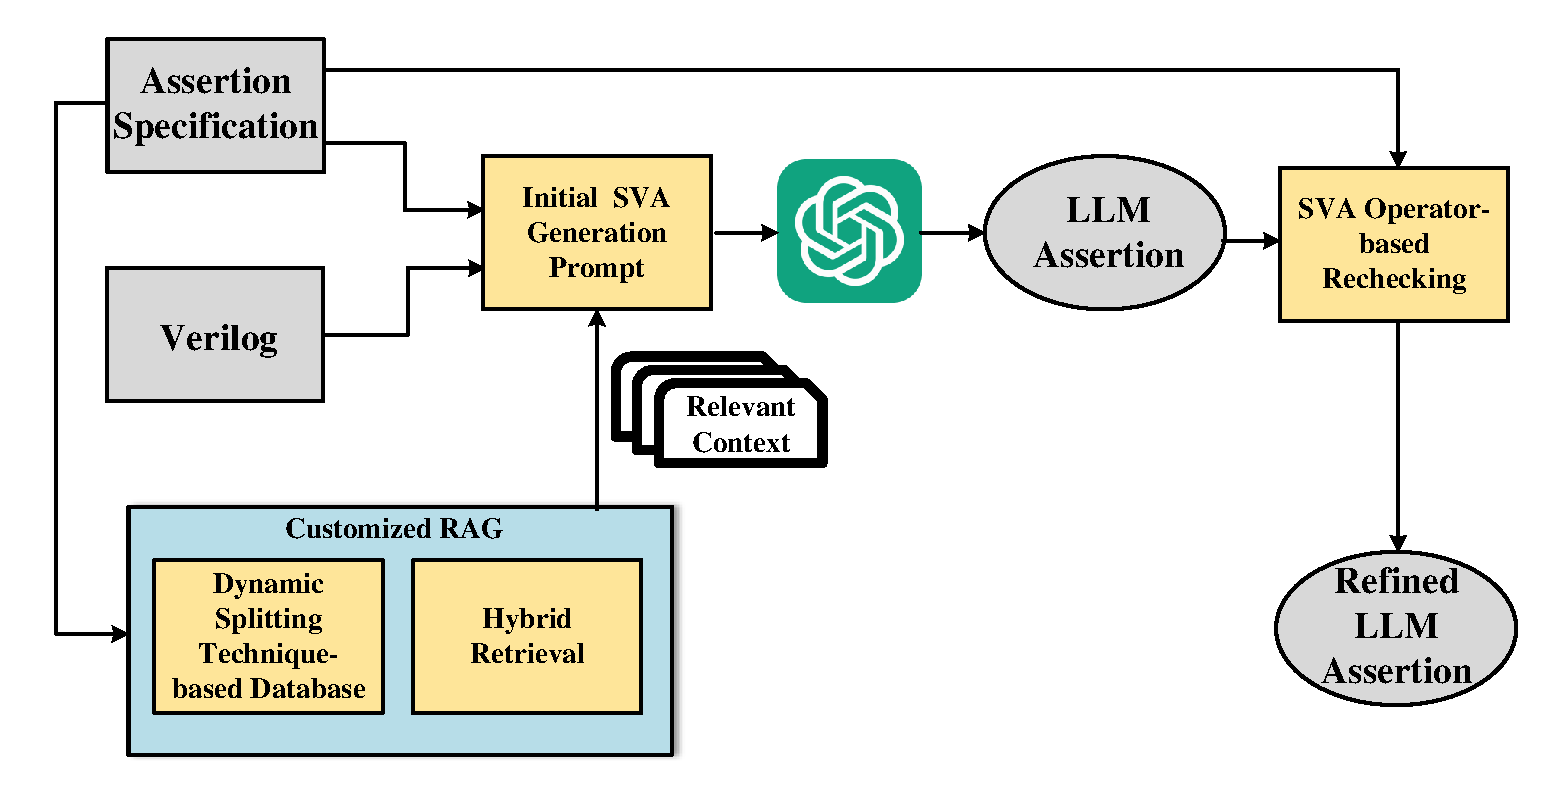
\includegraphics[width=\linewidth]{Figs/RAGSVAG.pdf}
    \caption{
    Overall flow of the proposed customized RAG framework: apply the proposed dynamic splitting to construct the database; apply the proposed HybridRetrieval to extract relevant context; apply the proposed SVA operator-based rechecking for correcting errors in generated SVAs.
    %Overall flow of the proposed RAGSVAG. {\bf Explain the flow here. You have two blocks with same name "Assertion Spec"  -->redraw to combine.}
    }
    \label{fig:overallflow-RAGSVAG}
\end{figure}
\subsubsection{Dynamic Splitting}
\label{subsubsec:Dynamic-Splitting}
addresses a key limitation of static splitting by distinguishing between code blocks and their related text. Instead of segmenting all content uniformly based on a fixed size threshold, our method constructs a specialized \textit{code database} designed to preserve the context surrounding each example.

The splitting process begins by parsing SystemVerilog textbooks to locate and isolate code snippets. 
% A \textit{font-based detection} is employed to recognize lines formatted in a distinctive style, such as a monospace font like \textit{Courier}. 
Whenever a code block is detected, the system automatically gathers the paragraph immediately preceding the code and the paragraph immediately following it. 
These three elements, consisting of the paragraph before, the code snippet itself, and the paragraph after, are combined into a single chunk, called \textit{code-centric chunk}. 
% This packaging ensures that the code snippet and its surrounding context, which is highly likely to be relevant to the code or its explanation, are preserved together within the same retrieval chunk.
% By packaging the code snippet together with its surrounding paragraphs, the local context that describes or references the code is preserved within the same retrieval unit.
Code-centric chunks are retained to construct the code database. 
Paragraphs not adjacent to a code snippet are not separately stored. 
% During retrieval, the system queries this code database to obtain relevant code examples along with their immediate natural language explanations.
By splitting content in this semantically-aware manner and focusing retrieval on code-centric contexts, dynamic splitting improves the relevance and precision of retrieved knowledge.
\subsubsection{HybridRetrieval}
\label{subsubsec:HybridRetrieval}
In addition to limitations in database construction, the retrieval process itself presents significant challenges when applying the basic RAG framework to SVA generation. Standard retrieval mechanisms based on global semantic similarity of the input prompt fail to capture fine-grained semantic embedded in natural language property specifications. Temporal relationships and operator-specific behaviors may be overlooked, resulting in the retrieval of incomplete or irrelevant contexts.

To address this issue, we propose \textit{HybridRetrieval}, a two-path retrieval mechanism that enhances context relevance by combining global semantic retrieval with keyword-guided operator retrieval. The overall flow is illustrated in Fig.~\ref{fig:HybridRetrieval}.
Given a natural language assertion specification, HybridRetrieval initiates two retrieval paths in parallel.
\begin{itemize}
    \item In the first path, a standard basic RAG retrieval is performed by embedding the entire input specification and retrieving chunks from the constructed code database based on global semantic similarity. 
    This step captures relevant contextual information corresponding to the global semantic of the property description.
    \item In the second path, the LLM is sequentially instructed with two custom prompts to extract fine-grain operator-related context. 
\end{itemize}
\begin{figure}
    \centering
    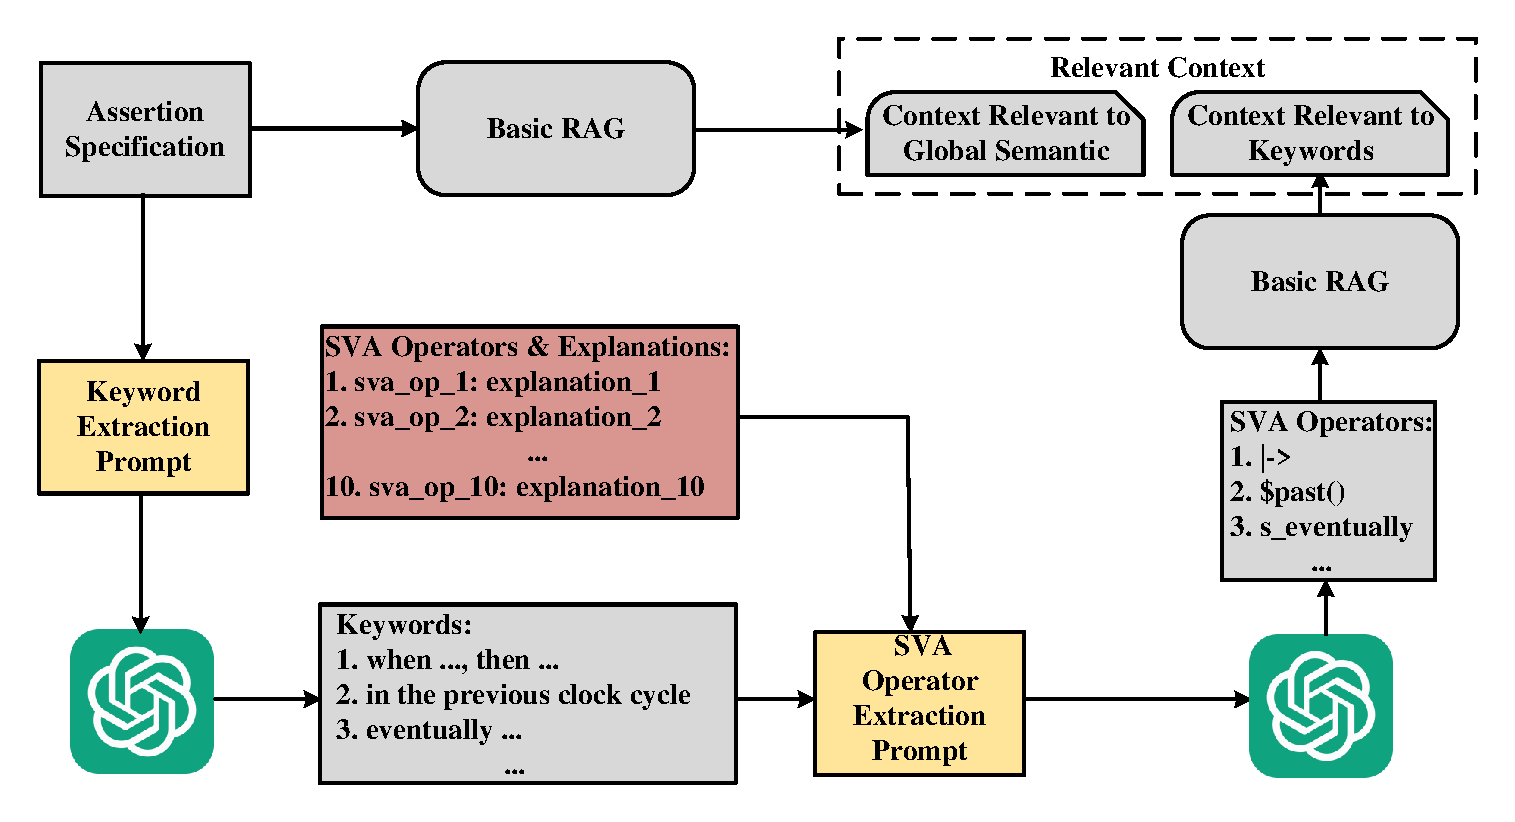
\includegraphics[width=\linewidth]{Figs/HybridRetrieval.pdf}
    \caption{Flow of HybridRetrieval combines the global semantic retrieval and the keyword-guided operator retrieval.}
    \label{fig:HybridRetrieval}
\end{figure}

The first prompt is the \textit{Keyword Extraction Prompt}. 
It instructs the LLM to decompose the natural language description of the assertion into multiple parts, each representing an operation over a single signal or a group of signals.
Examples of such keywords include phrases like \texttt{in the previous clock cycle}, which indicate the presence of temporal relationships between signals.
The keyword extraction prompt is shown in Fig.~\ref{fig:keyword_extraction_prompt}.
\begin{figure}
    \centering
    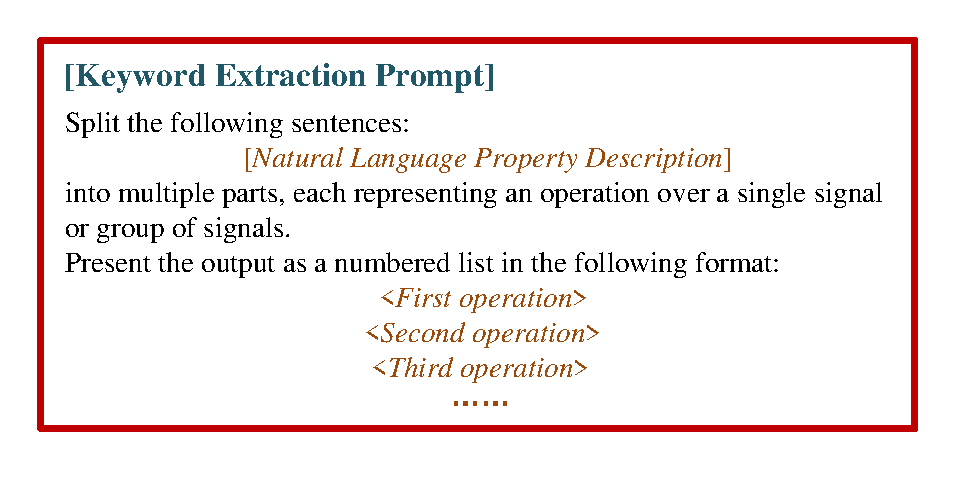
\includegraphics[width=\linewidth]{Figs/Keyword-Extraction.pdf}
    \caption{Keyword extraction prompt.}
    \label{fig:keyword_extraction_prompt}
\end{figure}
% \begin{framed}
% \begin{verbatim}
% // Keyword Extraction Prompt
% Split the following sentence: 
% ...... 

% into multiple parts, each representing 
% an operation over a single signal or 
% group of signals. 

% Present the output as a numbered list 
% in the following format:

% <First operation>
% <Second operation>
% <Third operation>
% ......
% \end{verbatim}
% \end{framed}

The second prompt is the \textit{SVA Operator Extraction Prompt}, which is then used to instruct LLM to map each extracted keyword to the most relevant SVA operator.
% To control the complexity and accuracy of mapping process, we construct a \textit{SVA Quick Reference Table} and instruct the LLM to map the most relevant operator from it.
To balance the complexity and accuracy of the mapping process, we prompt the LLM to select the most relevant operator from the $10$ SVA operators shown in Table~\ref{tab:sequence_sva_operators} and Table~\ref{tab:property_sva_operators}.
% To balance the complexity and accuracy of the mapping process, we construct an \textit{SVA Quick Reference Table}, consisting of a set of SVA operators and their corresponding natural language explanations, and prompt the LLM to select the most relevant operator from it.
% The SVA quick reference table is constructed by selecting ten commonly used SVA temporal operators, shown in Table~\ref{tab:sva_operators}.
% by referencing our constructed SVA quick reference table in Table~\ref{tab:sva_operators}. 
% The SVA quick reference table is constructed by selecting the ten commonly used SVA temporal operators.
The SVA operator extraction prompt is shown in Fig.~\ref{fig:sva_operators_extraction_prompt}.
\begin{figure}
    \centering
    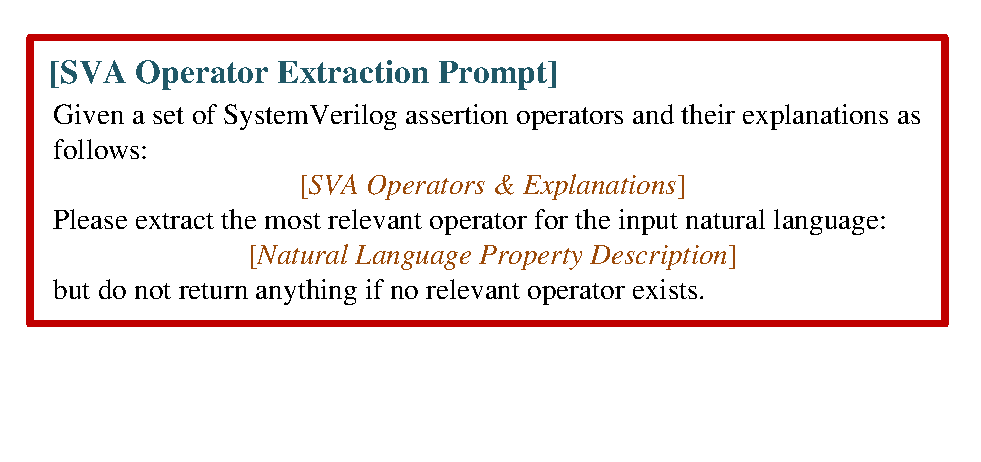
\includegraphics[width=\linewidth]{Figs/SVA-Operator-Extraction.pdf}
    \caption{SVA operators extraction prompt.}
    \label{fig:sva_operators_extraction_prompt}
\end{figure}
% \begin{framed}
% \begin{verbatim}
% // SVA Operator Extraction Prompt
% Given a set of SystemVerilog assertion 
% operators and their explanations as 
% follows: 
% ......

% Please extract the most relevant 
% operator for the input natural 
% language:
% ......

% but do not return anything if no 
% relevant operator exists.
% \end{verbatim}
% \end{framed}

Once the relevant SVA operators are identified, a RAG retrieval is conducted. 
This retrieval  targets database chunks that mention or explain the identified operators, ensuring that the retrieved context is not only semantically relevant but also aligned with the SVA operator semantics necessary for correct assertion construction.

Finally, the outputs from the global semantic and the operator-guided retrievals are combined with the initial SVA generation prompt to enrich the prompt. 
By integrating both the property semantics and operator-specific contexts, HybridRetrieval can improve the quality and completeness of information for the LLM during SVA generation.

% In addition to limitations in database construction, the retrieval process itself presents significant challenges when applying basic RAG frameworks to SVA generation. Standard retrieval mechanisms based purely on global semantic similarity often fail to capture fine-grained cues embedded in natural language property specifications. 
% Specifically, temporal relationships and operator-specific behaviors may be overlooked, leading to the retrieval of incomplete or irrelevant contexts.

% To address this limitation, we propose HybridRetrieval, which integrates global semantic retrieval with keyword-guided retrieval to enhance the specificity of retrieved knowledge. 
% As illustrated in Fig.~\ref{fig:HybridRetrieval}, the retrieval process begins with an initial prompt that describes a natural language property. 
% A global semantic retrieval first selects database chunks that are broadly related to the meaning of the prompt based on embedding similarity, which is just the same as the retrieval in basic RAG.

% Simultaneously, a keyword extraction stage is initiated. Using a lightweight LLM prompt, critical temporal or behavioral keywords are extracted from the input description. Examples of such keywords include phrases like "when..., then..." or "in the previous clock cycle," which suggest the presence of temporal dependencies. 
% These extracted keywords are then mapped to corresponding SystemVerilog operators, such as $|$\verb|->|, \verb|$past()|, or \verb|s_eventually|, using a curated operator reference table.
% This mapping process

% A second retrieval pass focuses specifically on locating database chunks that mention the identified SVA operators. By combining the results of both the global semantic search and the operator-guided search, HybridRetrieval forms an enriched set of contexts. This hybrid strategy ensures that the retrieved material captures both the overall semantic meaning of the input property and the specific temporal constructs critical for generating accurate SystemVerilog Assertions.


% \begin{table}[t]
% \centering
% \caption{SVA Quick Reference Table in RAGSVAG}
% \label{tab:sva_operators}
% \begin{tabular}{|c|c|}
% \hline
% \textbf{SVA Operator} & \textbf{Explanation} \\ \hline
% \texttt{\$rose} & \tabincell{l}{Detects that the condition transitions from false to \\true (rising edge).} \\ \hline
% \texttt{\#\#$n$} & \tabincell{l}{Delay operator that postpones evaluation by $n$ \\clock cycle.} \\ \hline
% \texttt{\$stable} & \tabincell{l}{Ensures that the signal value remains unchanged\\ during the evaluation cycle.} \\ \hline
% \texttt{|->} & \tabincell{l}{Overlapping implication operator, meaning that\\ if the conditions on the left are met, the condition\\ on the right must hold in the same clock cycle.} \\ \hline
% \texttt{\$isunknown} & Checks if a signal has an unknown (X or Z) value. \\ \hline
% \texttt{s\_eventually} & \tabincell{l}{Temporal operator indicating that the contained\\ condition is required to occur at some future\\ clock cycle.} \\ \hline
% \texttt{\$onehot0} & \tabincell{l}{Function that checks that no more than one bit\\ of the operand is set to 1.} \\ \hline
% \texttt{|=>} & \tabincell{l}{Non-overlapping implication operator, meaning \\that if the conditions on the left are met, the \\condition on the right must hold in the next\\ clock cycle.} \\ \hline
% \texttt{\$onehot} & \tabincell{l}{Function that verifies that exactly one bit in the \\operand is set to 1.} \\ \hline
% \texttt{\$past} & Refers to the value from previous clock cycle(s). \\ \hline
% \end{tabular}
% \end{table}

\subsubsection{SVA Operator-based Rechecking}
\label{subsubsec:SVA-Op-based-Rechecking}
Even with the improved retrieval through HybridRetrieval, LLMs may generate assertions that misuse SVA operators. 
Misinterpretations occur because retrieved materials, although relevant, may contain both helpful and noisy information. 
Certain SVA operators exhibit slight semantic differences, such as \texttt{|->} and \texttt{|=>}, that are difficult for LLMs to distinguish during initial generation, particularly regarding precise timing and logical behavior.

To address these challenges, we propose an SVA operator-based rechecking flow. 
% Given a LLM generated assertion, a rechecking stage is introduced to check the functional correctness of the generated assertion with respect to the original natural language property description.
In this stage, the flow first extracts the list of operators present in the generated assertion. 
The relevant explanations for these operators are then retrieved from Table ~\ref{tab:sequence_sva_operators} and Table~\ref{tab:property_sva_operators}. 
Given these context, the \textit{SVA Rechecking Prompt} is applied to instruct the LLM to verify the correct use of SVA operators in the LLM-generated assertion. 
The SVA rechecking prompt is shown in Fig.~\ref{fig:SVA_Checking_Prompt}.
\begin{figure}
    \centering
    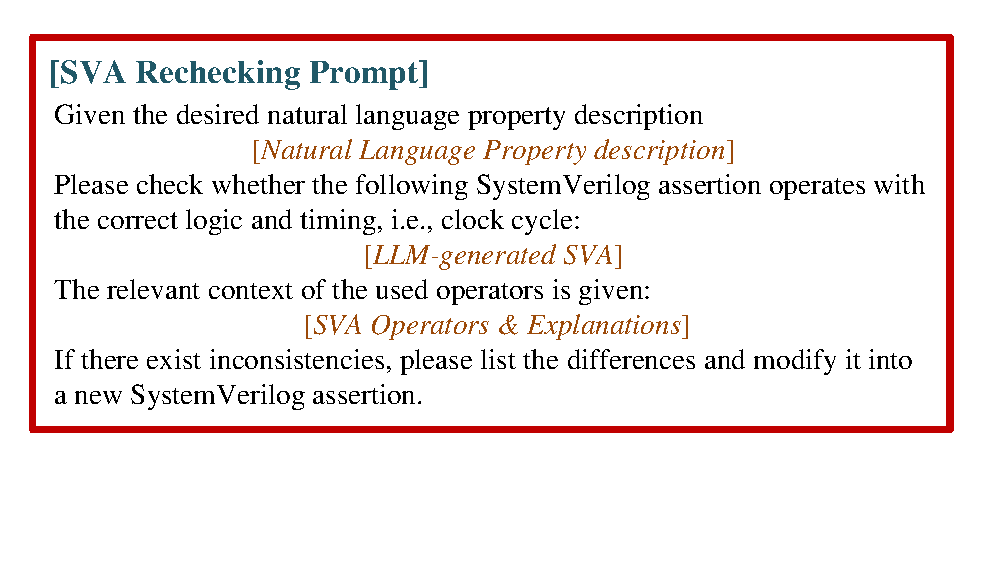
\includegraphics[width=\linewidth]{Figs/SVA-Rechecking.pdf}
    \caption{SVA checking prompt.}
    \label{fig:SVA_Checking_Prompt}
\end{figure}
% \begin{framed}
% \begin{verbatim}
% // SVA Rechecking Prompt
% Given the desired natural language 
% property description 
% ......

% Please check whether the SystemVerilog 
% assertion 
% ......

% operates with the correct logic and 
% timing (i.e., clock cycle).

% The relevant context of the used 
% operators is given: 
% ...... 

% If there exist inconsistencies, please 
% list the differences and modify it 
% into a new SystemVerilog assertion.
% \end{verbatim}
% \end{framed}

% By incorporating the operator-based rechecking flow, the framework enhances the correctness of SVA operator usage and improves the overall quality of LLM-generated assertions.

% Even with improved retrieval through HybridRetrieval, LLMs may still generate assertions that misuse SystemVerilog operators. Misinterpretations often occur because retrieved materials, although relevant, may contain both helpful and noisy information. Additionally, certain SVA operators exhibit subtle semantic differences that are difficult for LLMs to distinguish during initial generation.

% To further improve the functional correctness of generated assertions, we propose an SVA operator-based rechecking flow, as illustrated in Fig. 2. After the LLM generates an initial assertion, the system first extracts the list of SVA operators present in the assertion text. Each extracted operator is cross-checked against an SVA operator reference, which provides a concise description of its intended behavior and temporal semantics.

% A rechecking prompt is then constructed, incorporating both the original natural language description and the generated assertion. The LLM is tasked with verifying whether the assertion correctly reflects the intended functionality of the identified operators. If inconsistencies or mismatches are found between the operator semantics and the assertion behavior, the LLM is instructed to revise and correct the assertion accordingly.

% This operator-based rechecking flow serves as a post-generation refinement step that ensures not only syntactic correctness but also deeper semantic alignment between the natural language property description and the formal SVA expression.
% \begin{figure}
%     \centering
%     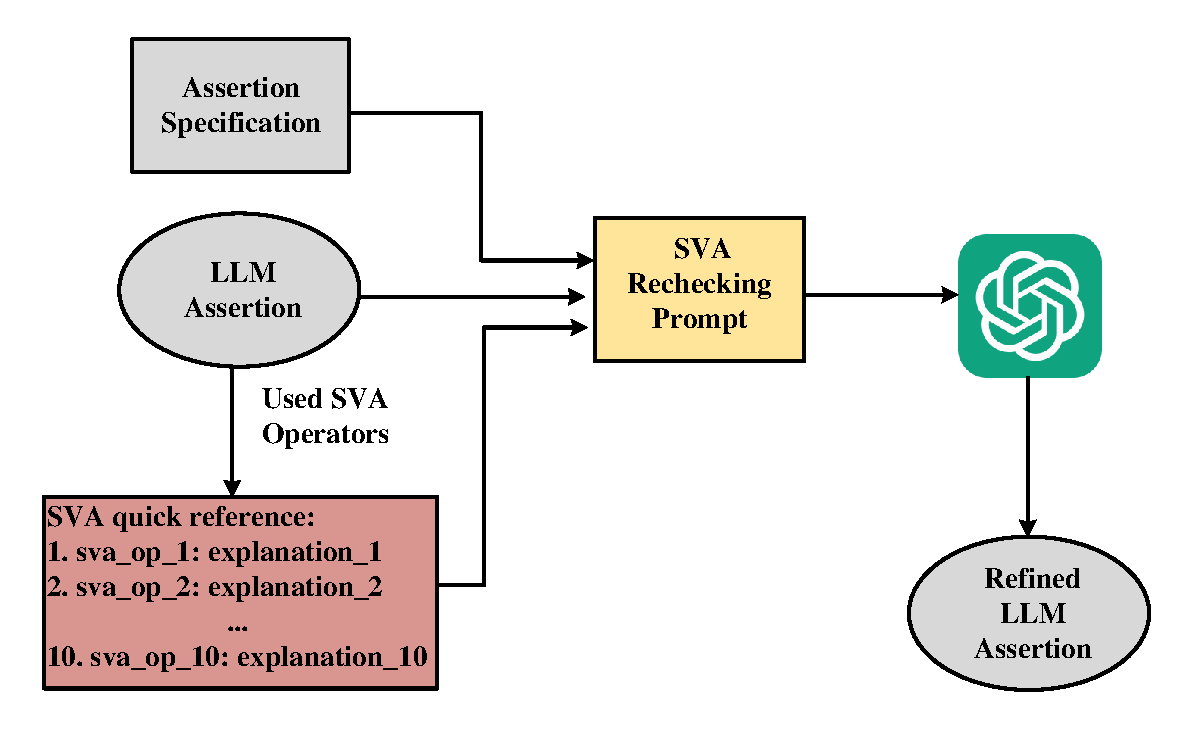
\includegraphics[width=\linewidth]{Figs/SVAOperatorRefine.pdf}
%     \caption{Flow of SVA operator-based rechecking.}
%     \label{fig:SVA-Rechecking}
% \end{figure}
\subsection{Synthetic Finetuning Dataset for NL2SVA}
\label{subsec:synthetic-finetuning-dataset}
Although Section ~\ref{subsec:RAGSVAG} introduces a customized RAG framework for guiding LLMs to do NL2SVA, lightweight LLMs may struggle to follow the different chained prompts in that pipeline. 
Their shorter context windows can also truncate the combined prompt and retrieved context, leading to incomplete or incoherent output. 
To overcome these limits, we prepare a supervised fine-tuning dataset that teaches smaller models to perform the NL2SVA task directly, without relying on long, multi-stage prompts.

By scraping Verilog codes from $67$ hardware-design textbooks spanning digital logic, computer architecture, SoC implementation, and formal verification, and extracting every embedded SVA, we obtained $4070$ ground-truth assertions.
Each assertion is paired with a concise, one-sentence natural language explanation produced by prompting \textit{OpenAI o4-mini} with the raw SVA and natural language explanations of SVA operators (Table~\ref{tab:sequence_sva_operators} and Table~\ref{tab:property_sva_operators}).
% For every assertion we then obtain a concise, one-sentence English description. \textit{OpenAI o4-mini} model receives the raw SVA together with a short glossary of SVA operators (Table 1) and is instructed to return a single behavioural statement. Because the prompt enforces length and style constraints, the resulting explanations are uniform and fit well within the context window of lightweight models.

The core feature of our fine-tuning dataset is a complete layer-by-layer derivation trace of each SVA from its corresponding natural language explanation. 
We refer to this trace as a \textit{Prompt-guided Explanation}. 
Section~\ref{subsec:SVA} describes the four layers of a concurrent SVA, and the prompt-guided explanation records how those layers are actually constructed for each individual case. 
The prompt-guided explanation is produced by OpenAI o4-mini. We feed each pair of the SVA and explanation to the LLM and instruct it to reconstruct the SVA from the explanation step by step as follows:
\begin{itemize}
    \item [(1)] Identify the top-level property SVA operator.
    \item [(2)] Split the natural language explanation into operand fragments that match the number of operands of the selected operator;
    \item [(3)] For each fragment, decide whether it represents a sequence or a property. If it is a sequence, translate it into a sequence expression directly; otherwise, recursively apply Steps $1$--$4$.
    \item [(4)] Combine the fragment expressions into the complete property expression using the selected property SVA operator.
    \item [(5)] Wrap the property expression in \texttt{assert property (...)}.
\end{itemize}
The detailed prompt for generating the prompt-guided explanation is shown in Appendix~\ref{subsec:prompt-guided-explanation-generation} and an example prompt-guided explanation is shown in Appendix~\ref{subsec:example-prompt-guided-explanation}.
\subsection{Evaluation Dataset}\label{subsec:Evaluation-Dataset}
In constructing our evaluation dataset, we aim to ensure both realism and quality in the SVAs. 
To achieve this, we gather $40$ Verilog designs and $229$ concurrent SVAs from a combination of open-source cores and academic verification courses. 
In Fig.~\ref{fig:sva-ops-signals}, it summarizes the operator and signal counts for all $229$ SVAs, showing the complexity of each SVA and indicating that most of them are non-trivial.

Each of them is verified to ensure syntax and functionality correctness using FPV tool \textit{Cadence JasperGold}~\cite{cadencejaspergold}. 
The evaluation dataset provides the  natural language property for each SVA, which is generated manually.
Note that each explanation does not contain any detailed signals, which are translated as natural language descriptions.
In Appendix~\ref{subsec:Example-SVAs}, it shows $10$ example natural language properties from our evaluation dataset. 
\begin{figure}
    \centering
    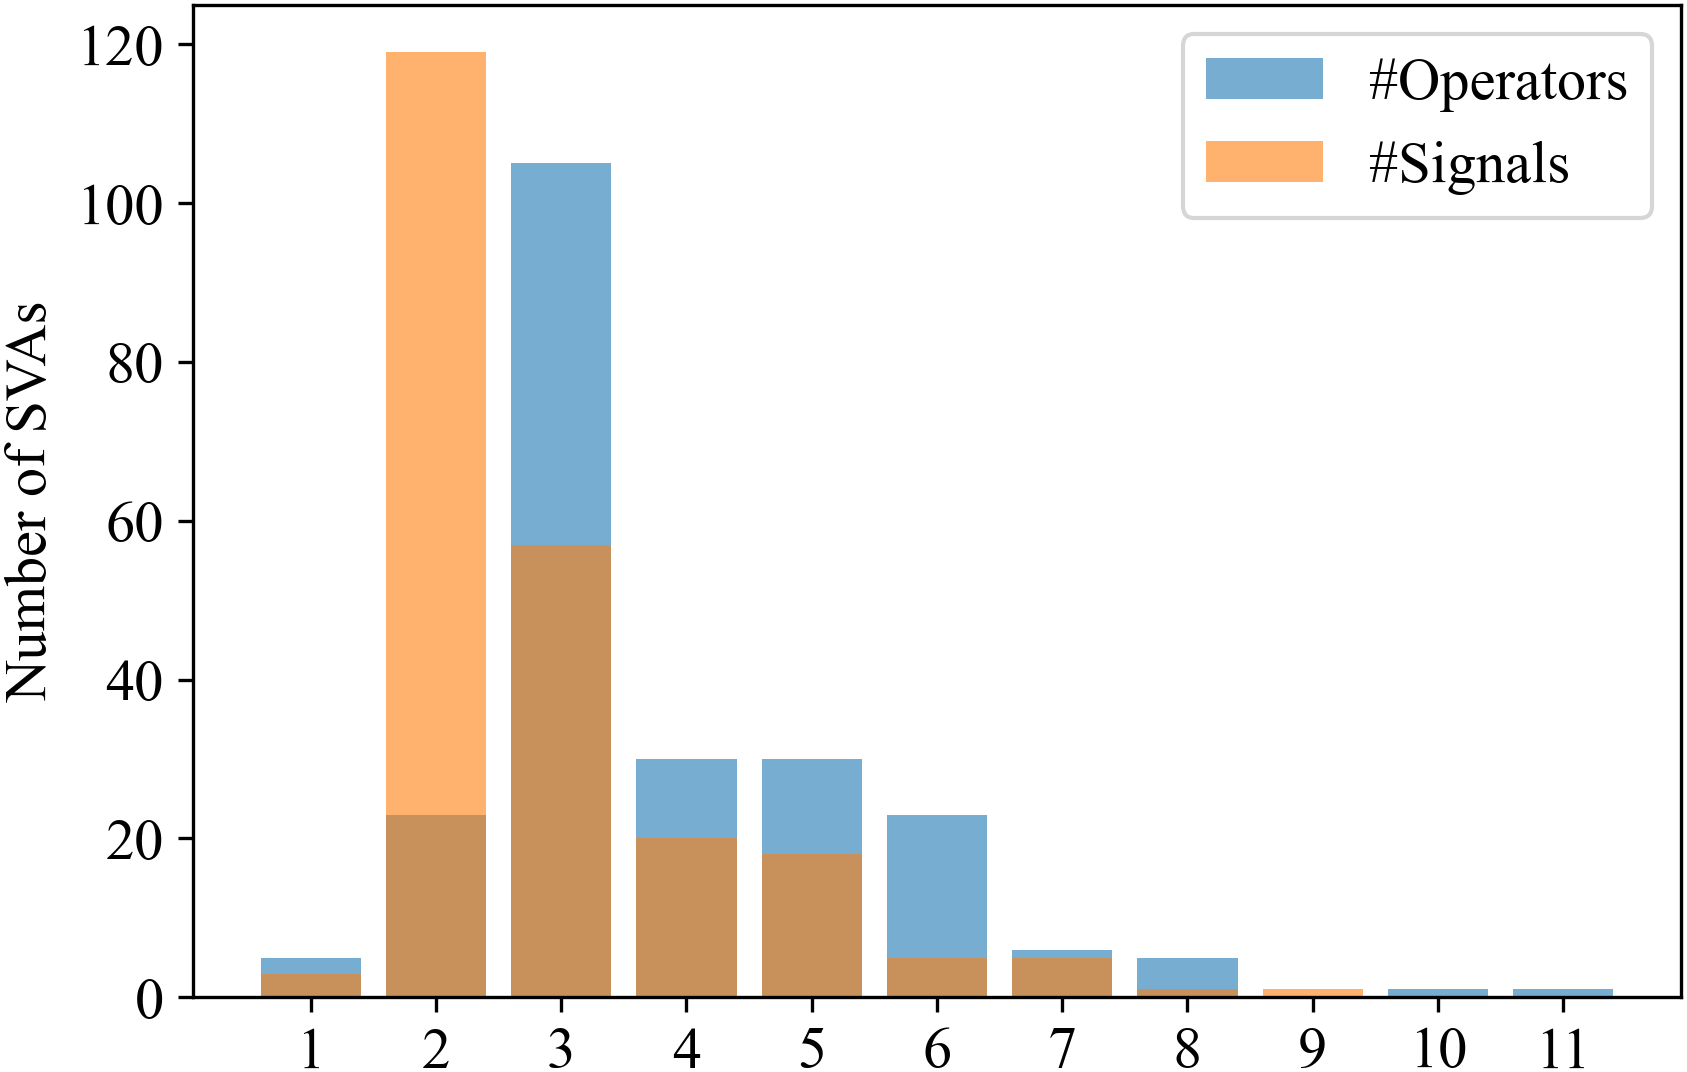
\includegraphics[width=0.9\linewidth]{Figs/op_signal_statistics.png}
    \caption{Number of SVA operators and signals in the $229$ SVAs.}
    \label{fig:sva-ops-signals}
\end{figure}
% These assertions are then subjected to a three-step validation process using the \textit{formal property verification} (\textit{FPV}) tool \textit{Cadence JasperGold}~\cite{cadencejaspergold}. 
% First, we check syntax correctness to confirm that each assertion is syntactically valid and could be parsed by the tool. 
% Second, we verify functionality correctness by running formal proofs on the designs and their corresponding assertions, ensuring that no counterexamples are generated.
% % Second, we test functionality correctness by running formal proofs on the designs and each assertion; no counterexamples are allowed to exist. 
% Some assertions use implication operators, which do not check properties unless the precondition is met as mentioned in Section~\ref{subsec:SVA}. 
% If there is no scenario that triggers the precondition, the assertion becomes meaningless. Third, in such situations, we examine whether the preconditions can be covered.
% Some assertions employ the implication operators. 
% As is mentioned in Section~\ref{subsec:SVA}, they will not check any properties when the precondition is not asserted.
% Thus, if there exists no case making the precondition assert, the assertion is meaningless.
% Third, in these cases, we check whether the preconditions can be covered.

% For each of the $40$ designs, we provide:
% \begin{itemize}
%     \item \textit{Verilog source code}: Verilog files that contain the RTL implementation of the design.
%     \item \textit{JSON file} that details each of the associated SVA:
%     \begin{itemize}
%         \item \textit{clock signal condition}
%         \item \textit{disable condition}
%         \item \textit{logical expression}
%         \item \textit{Signals}: a list of signals referenced by the assertion;
%         \item \textit{Assertion Explanation}: human-written explanation of the logic expression.
%     \end{itemize}
% \end{itemize}

% In Fig.~\ref{fig:example-evaluation-dataset}, it shows an example design \verb|register| and its associated JSON file from our evaluation dataset.
% The design has two associated SVAs, which can be extracted from the JSON file. 
% For example, the first assertion is 
% \begin{verbatim}
% assert property (@(posedge clk) 
%                  disable iff (rst) 
%                  en |=> out==$past(in,1));
% \end{verbatim}
% with the used signals \texttt{en}, \texttt{out}, \texttt{in}, and the human-written explanation: when enable signal is set (1), output 
% signal equals the last one clock cycle's 
% input signal from the next clock cycle.
% \begin{figure}
%     \centering
%     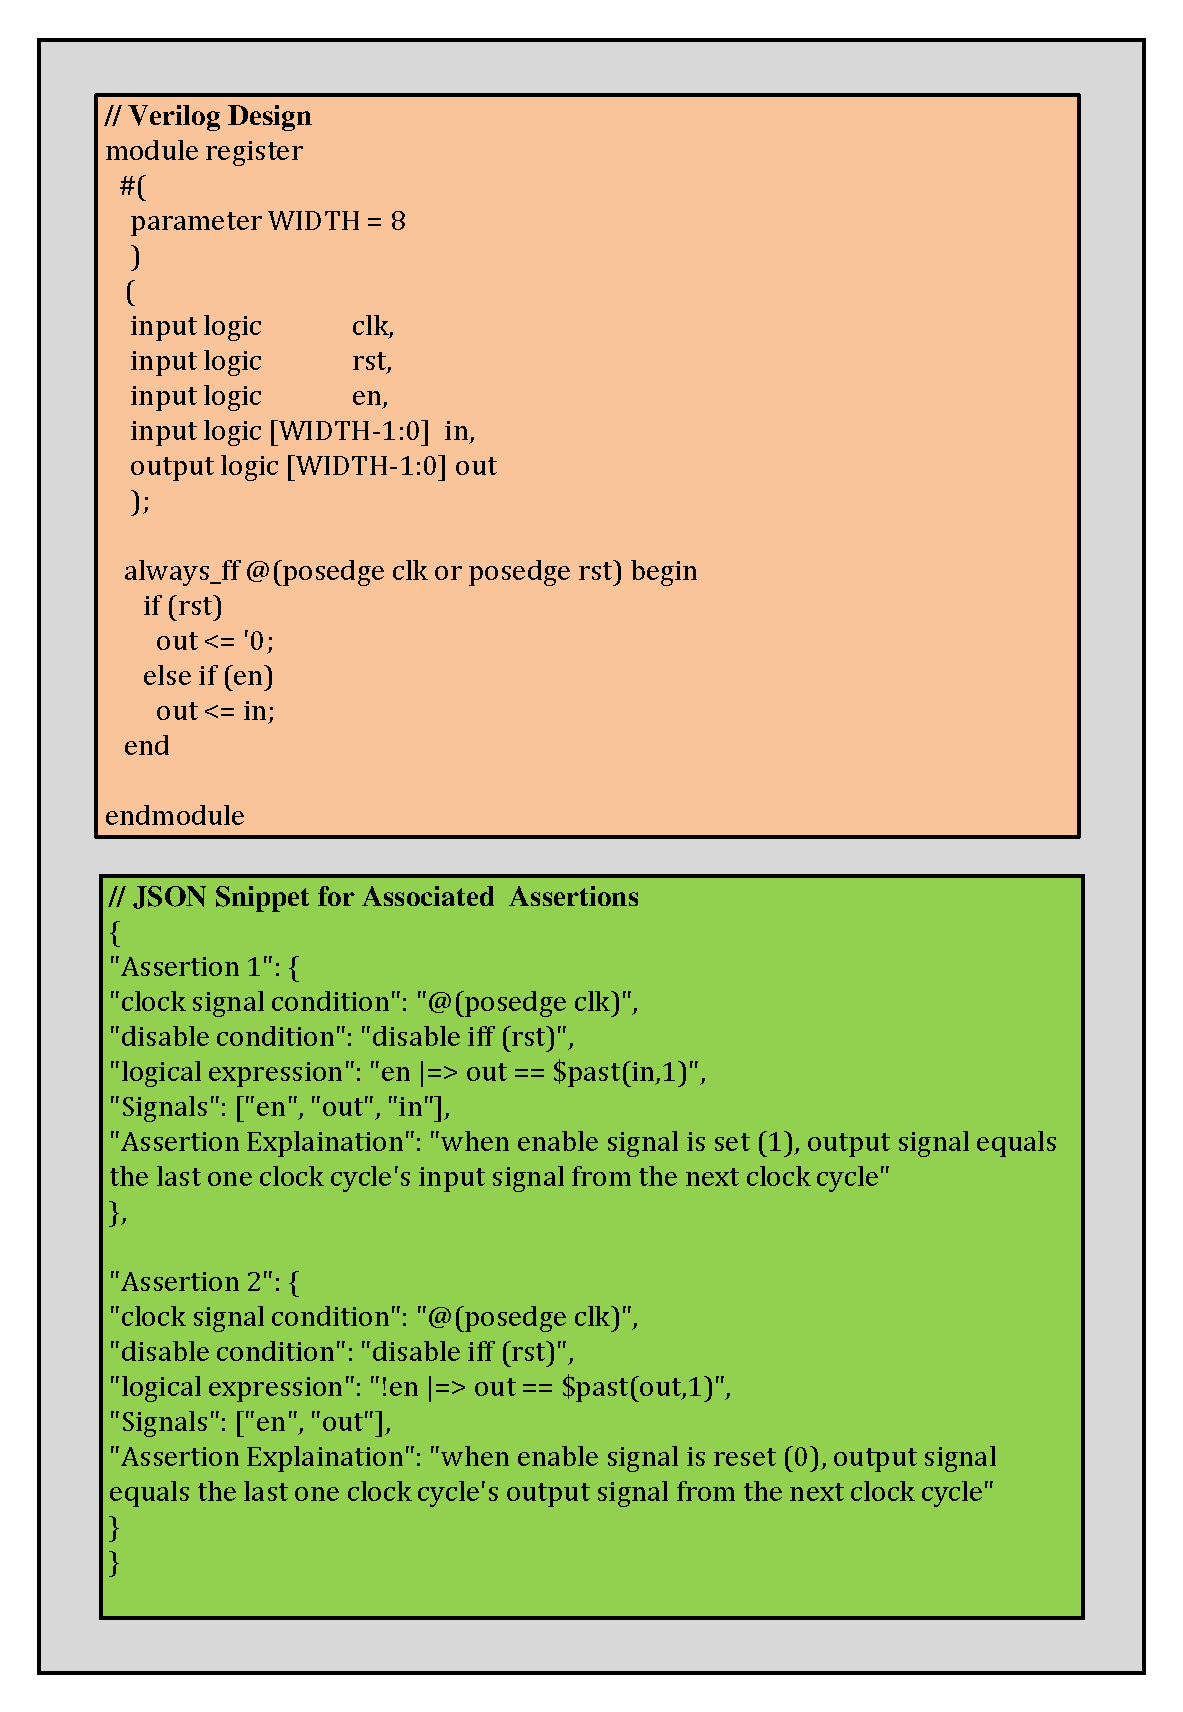
\includegraphics[width=1\linewidth]{Figs/Evaluation_Dataset.pdf}
%     \caption{An example Verilog design and the associated JSON file storing two SVAs and their corresponding details.}
%     \label{fig:example-evaluation-dataset}
% \end{figure}
% Implementation details
% are available in our repository\footnote{ https://github.com/FCHXWH823/RAG-aided-Assertion-Generation}.

% \begin{figure}
%     \centering
%     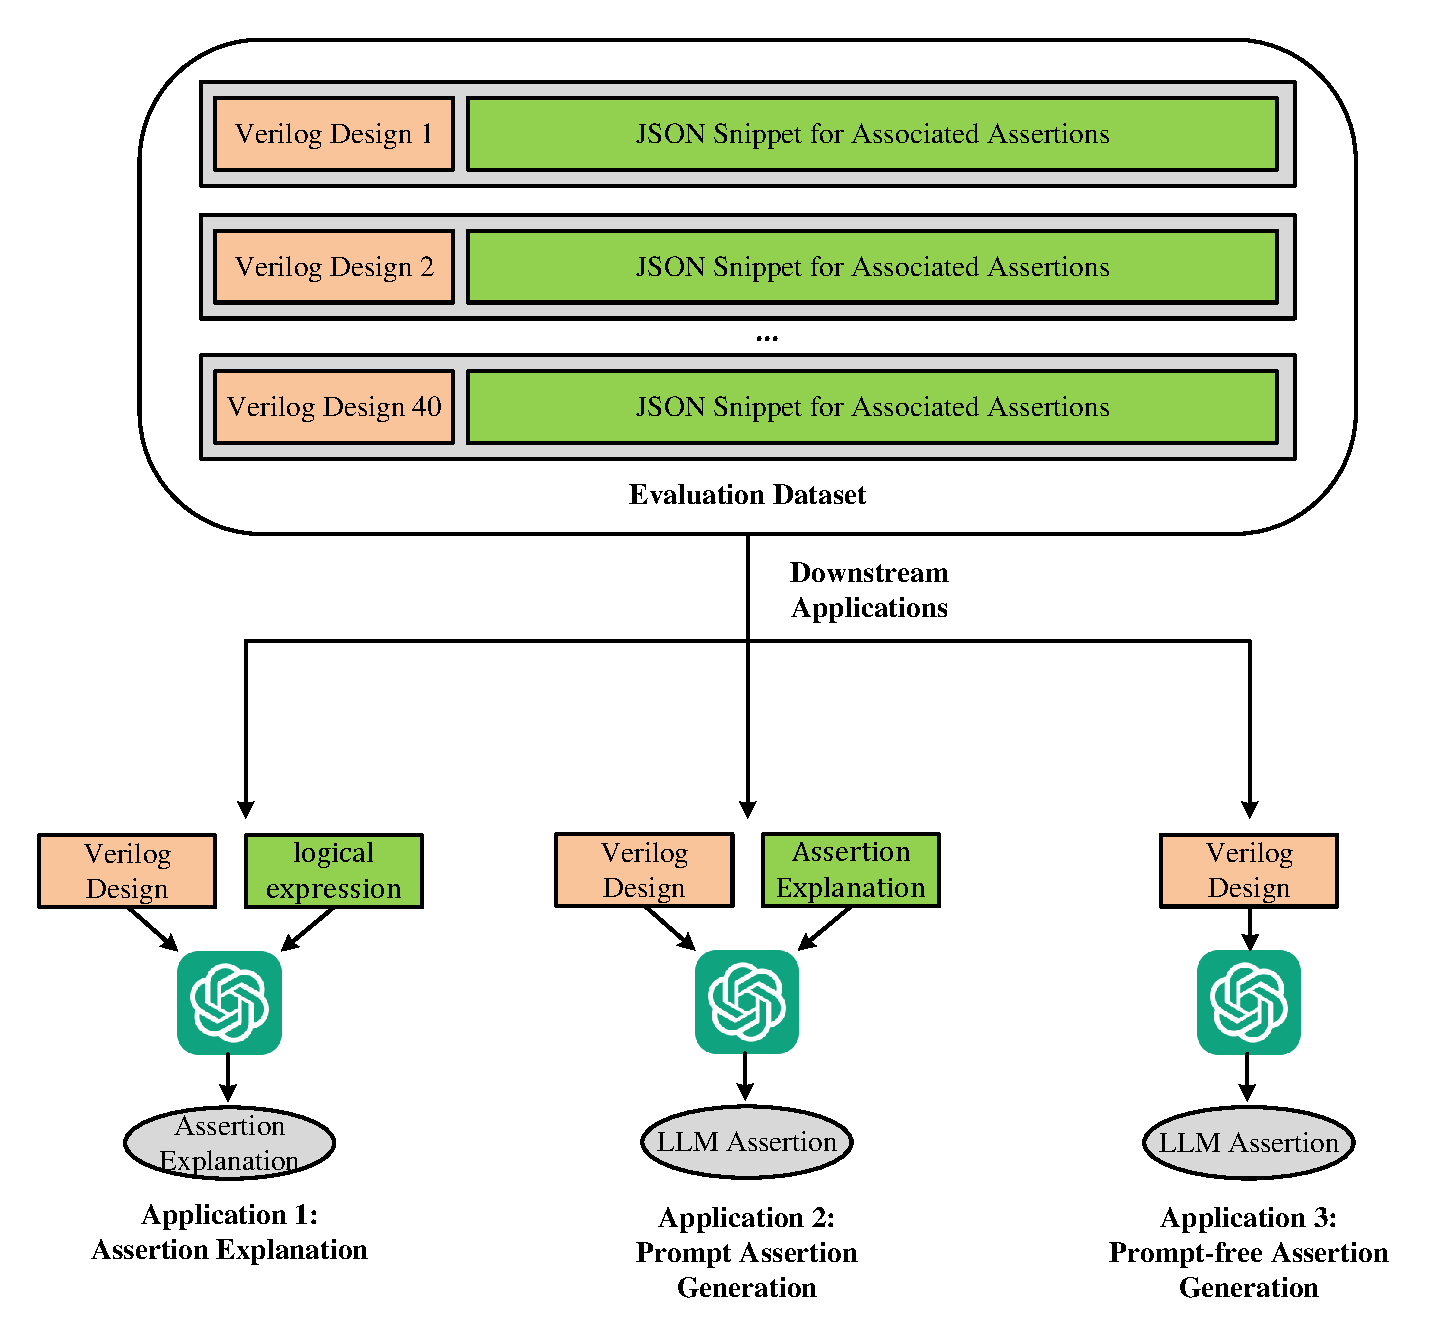
\includegraphics[width=\linewidth]{Figs/RAG_Downstream_Applications.pdf}
%     \caption{Support evaluating multiple downstream assertion-related tasks by the proposed evaluation dataset.}
%     \label{fig:down-stream-related-tasks}
% \end{figure}

% In Fig.~\ref{fig:down-stream-related-tasks}, our evaluation dataset supports assessing three different downstream assertion-related tasks because each assertion includes detailed annotations. 
% \begin{itemize}
%     \item \textit{Assertion Explanation}: In this task, the LLM is given an existing assertion along with the corresponding Verilog design context. 
%     The goal is to produce a human-readable explanation of what the assertion does.
%     This tests the LLM’s ability to interpret SystemVerilog syntax, understand the design’s functionality, and explain the purpose of a given property.
%     \item \textit{Prompt Assertion Generation}: the LLM is prompted with a natural language description of a property or behavior, along with relevant design context. 
%     The model must then generate the corresponding SVA. 
%     This scenario evaluates the LLM’s ability to map a natural language specification to the correct signals and syntaxes within an SVA, ensuring that the final assertion accurately captures the intended behavior.

%     \item \textit{Prompt-free Assertion Generation}:
%     the LLM receives only the Verilog design. 
%     It must output a meaningful set of assertions. 
%     This challenges the model to identify important design behaviors or corner cases on its own and encode them as SVAs. Evaluating performance on this task reveals how well the LLM can detect and formalize key properties from a design without explicit guidance.
%     \end{itemize}

% LLM-aided assertion generation is inherently challenging because it demands several distinct abilities.
% Our evaluation dataset enables a comprehensive evaluation of these different LLM abilities.
% This level of granularity is crucial for diagnosing which aspects of the LLM’s understanding or generation capabilities need further refinement, ultimately guiding targeted improvements in LLM-based assertion generation.

% Finally, an automatic evaluation framework is proposed to evaluate the effectiveness of our RAGSVAG.
% The pipeline begins with two key inputs: the Verilog design and its assertion specification, which are both from the evaluation dataset. 
% Then, our RAGSVAG receives the two inputs and outputs the corresponding SVA.
% % The two inputs are combined with the output assertion format to construct the \textit{initial prompt}. 
% % The template of the initial prompt is shown in Fig.~\ref{fig:Combined-Prompt}.
% Once the LLM assertion is generated, it is compared to a golden assertion from the evaluation dataset, which serves as the reference or ground-truth. 
% To verify that the two assertions are functionally equivalent, they are merged into a single assertion using the SVA operator \verb|iff|, which is then checked by the FPV tool. 
% If the FPV analysis reveals no counterexamples violating this combined assertion, the LLM assertion is functionally equivalent to the golden one.
% \begin{figure}
%     \centering
%     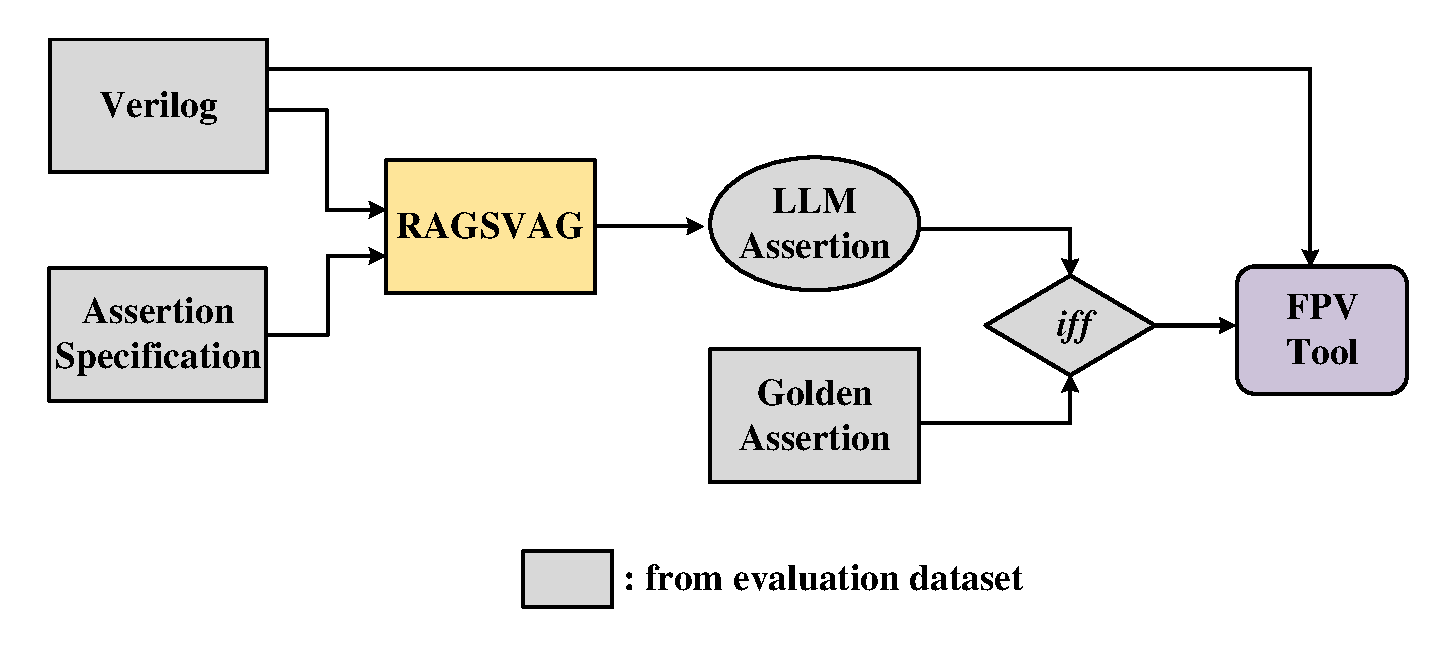
\includegraphics[width=\linewidth]{Figs/Verification_Flow.pdf}
%     \caption{Automatic evaluation framework for LLM-aided SVA generation from natural language.}
%     \label{fig:prompt-assertion-generation-framework}
% \end{figure}

% \subsection{RAG-aided Prompt Assertion Generation}
% \label{subsec:RAG-aided-Assertion-Generation}
% In this section, we aim at using RAG to improve the prompt assertion generation of LLM.

% First, an automatic evaluation framework is proposed for prompt assertion generation, shown in Fig.~\ref{fig:prompt-assertion-generation-framework}.
% The pipeline begins with two key inputs: the Verilog design and its assertion specification, which are both from the evaluation dataset. 
% The two inputs are combined with the output assertion format to construct the \textit{initial prompt}. 
% The template of the initial prompt is shown in Fig.~\ref{fig:Combined-Prompt}.
% Once the LLM assertion is generated, it is compared to a golden assertion from the evaluation dataset, which serves as the reference or ground-truth. 
% To verify that the two assertions are functionally equivalent, they are merged into a single assertion using the SVA syntax \verb|iff|, which is then checked by the FPV tool. 
% If the FPV analysis reveals no counterexamples violating this combined assertion, the LLM assertion is functionally equivalent to the golden one.

% % Once the LLM assertion is produced, it is compared against the golden assertion drawn from the evaluation dataset. 
% % This golden assertion serves as a reference or “ground truth,” ensuring that the assertion generated by the LLM should be functionality-equivalent to the golden one. 
% % The functionality-equivalent checking is realized by:
% % combining the LLM assertion and golden assertion into a new assertion using the SVA syntax \verb|iff|, which is then checked by the FPV tool; 
% % if there is no counterexamples violating the new combined assertion, the LLM assertion is equivalent to the golden one.

% \begin{figure}
%     \centering
%     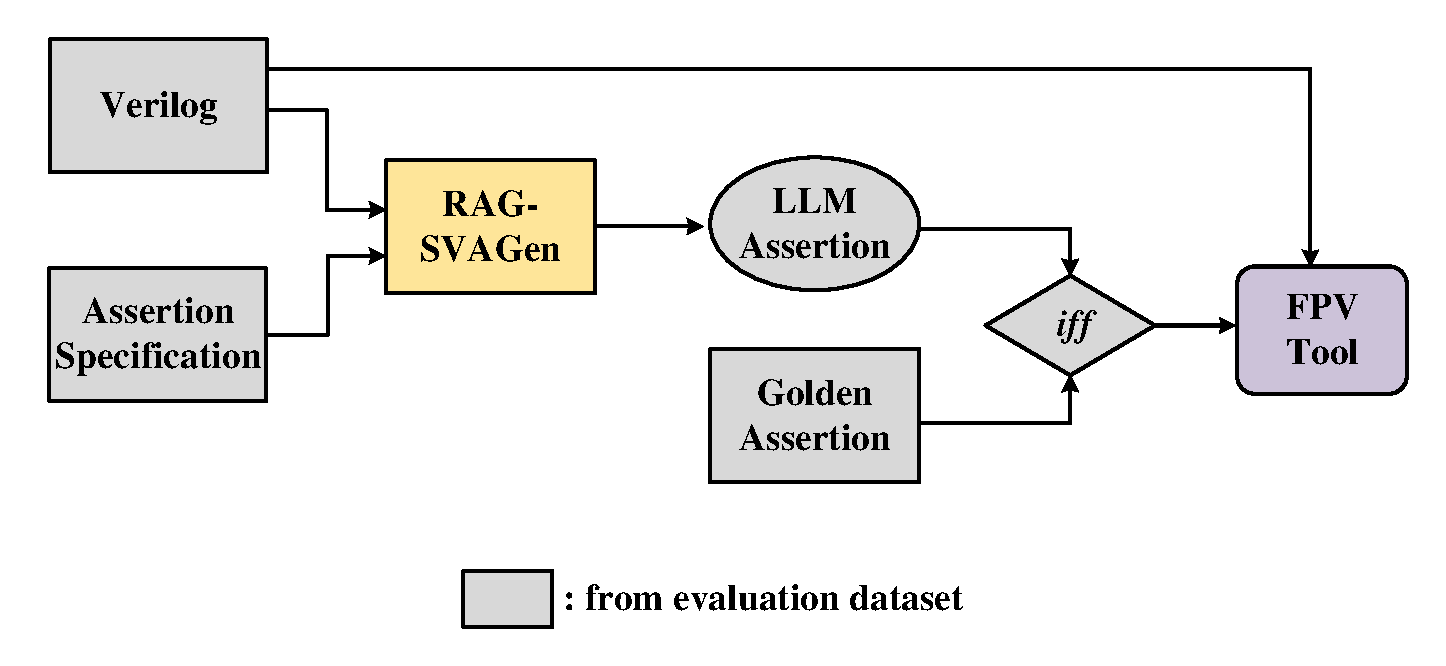
\includegraphics[width=\linewidth]{Figs/Prompt_Assertion_Generation_Flow.pdf}
%     \caption{Automatic evaluation framework for prompt assertion generation.}
%     \label{fig:prompt-assertion-generation-framework}
% \end{figure}

% Next, we will introduce our proposed framework using RAG to provide domain-specific context for prompt assertion generation. 
% As shown in Fig.~\ref{fig:RAG-Prompt-Assertion-Generation}, we construct a RAG database from Verilog textbooks by splitting the contents into chunks. 
% When an assertion specification is given, the RAG framework retrieves the most relevant chunks to augment the user’s initial prompt, ultimately forming a combined prompt that the LLM uses to generate the corresponding SVA. 
% Below, we introduce two proposed splitting techniques for better constructing the database.
% \subsubsection{Static Splitting Technique-based Database}
% In the static splitting approach, the Verilog textbook content is divided into chunks based on a fixed upper bound of characters per chunk. For instance, the text might be segmented every $1000$ characters, ensuring that each chunk remains within a manageable size for embedding and retrieval.
% % Extraction: We first extract the textbook content in its entirety, preserving paragraph boundaries where possible.
% % Chunking: Each block of text is split into pieces once it exceeds the character limit, creating chunks that are large enough to provide context but small enough for efficient retrieval.
% % Embedding and Indexing: Every chunk is converted into a vector embedding using an embedding model (e.g., a transformer-based encoder) and then stored in the RAG database with its metadata (e.g., the page number or section header).
% % Retrieval: At query time, the system calculates the embedding for the user’s prompt and performs a similarity search over all stored embeddings. The top-ranked chunks are retrieved and appended to the user’s initial prompt to form a combined prompt for the LLM.
% Although this method is straightforward and ensures a predictable chunk size, it may inadvertently split related concepts or code snippets, potentially scattering context across multiple chunks.
% \begin{figure}
%     \centering
%     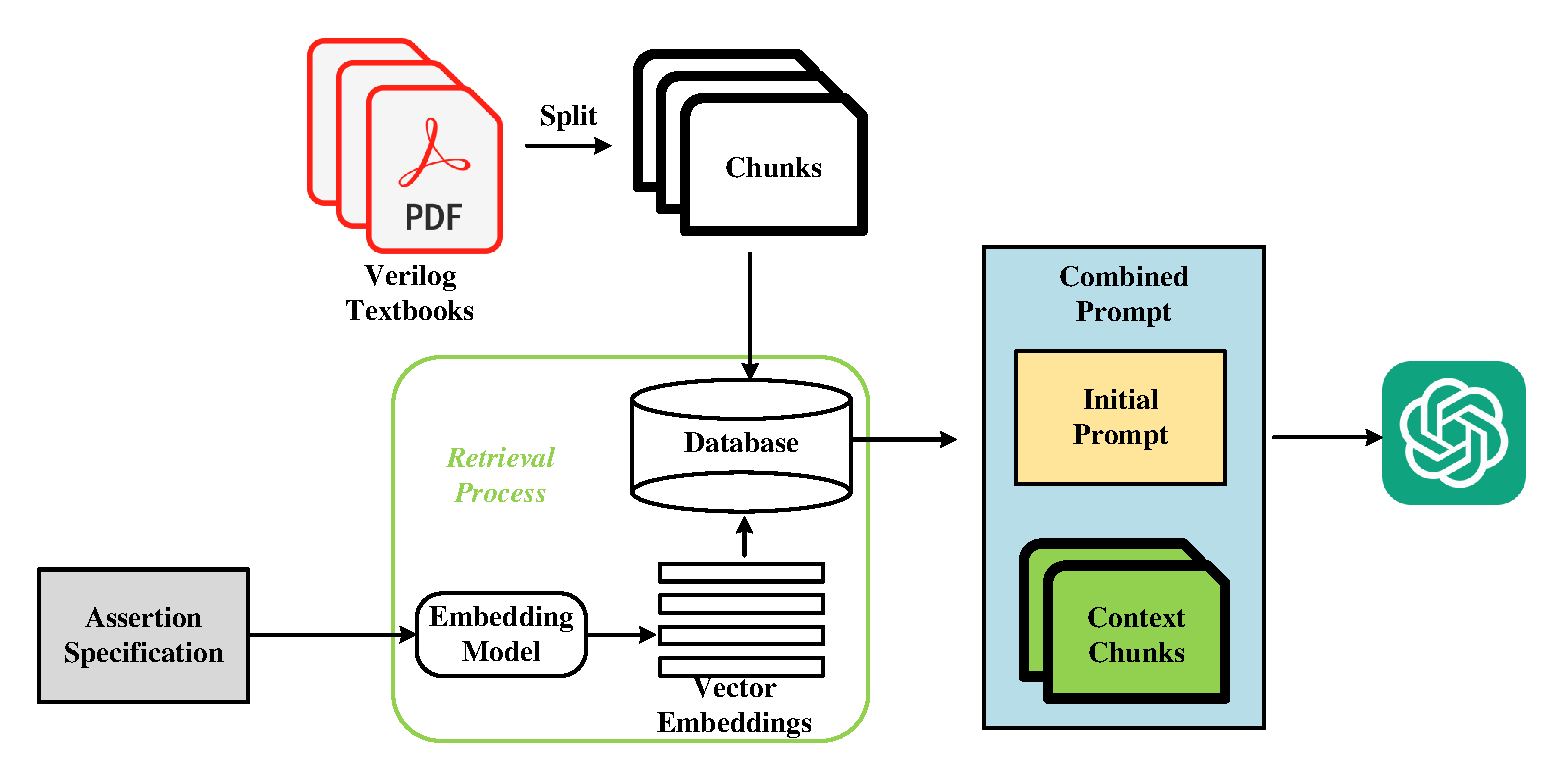
\includegraphics[width=\linewidth]{Figs/RAG_Prompt_Assertion_Generation.pdf}
%     \caption{Framework of RAG-aided prompt assertion generation.}
%     \label{fig:RAG-Prompt-Assertion-Generation}
% \end{figure}
% \subsubsection{Dynamic Splitting Technique-based Database}
% The dynamic splitting technique addresses a key limitation of the static approach by distinguishing between code blocks and explanatory text. 
% It constructs two databases: \textit{Code Database} and \textit{Text Database}.

% Rather than dividing all content at a uniform size threshold, this method begins by parsing the Verilog textbook to locate and isolate code snippets. 
% A font-based detection algorithm, for example, can recognize code segments displayed in a monospace font or other distinctive style. 
% The dynamic splitting technique scans the Verilog textbook for code snippets, using a font-based detection approach to identify lines formatted in a distinct font, such as \textit{Courier}.
% Whenever a code block is detected, it automatically gathers the paragraph immediately preceding the code and the paragraph immediately following it. 
% These three elements—one paragraph before, the code snippet, and one paragraph after—are then combined into a single chunk. By packaging the surrounding paragraphs together with the code, the chunk preserves the immediate context that explains or references the snippet, making it more likely to be useful during retrieval.

% All other text—paragraphs not adjacent to a code block—is split into individual paragraphs and placed in the text database. Each paragraph is processed as its own chunk, enabling the system to retrieve conceptual or theoretical explanations independently. When a user query arrives, the system decides which database to consult based on the query’s nature. If the request involves specific code syntax or an example usage, the code database is queried for the relevant snippet and its neighboring text. Conversely, if the user’s query is more conceptual, the system draws on the text database to provide the appropriate explanatory paragraph(s).

% By splitting content in this manner, the dynamic splitting technique captures local context around code blocks while also making higher-level explanations accessible.


% \begin{figure}
%     \centering
%     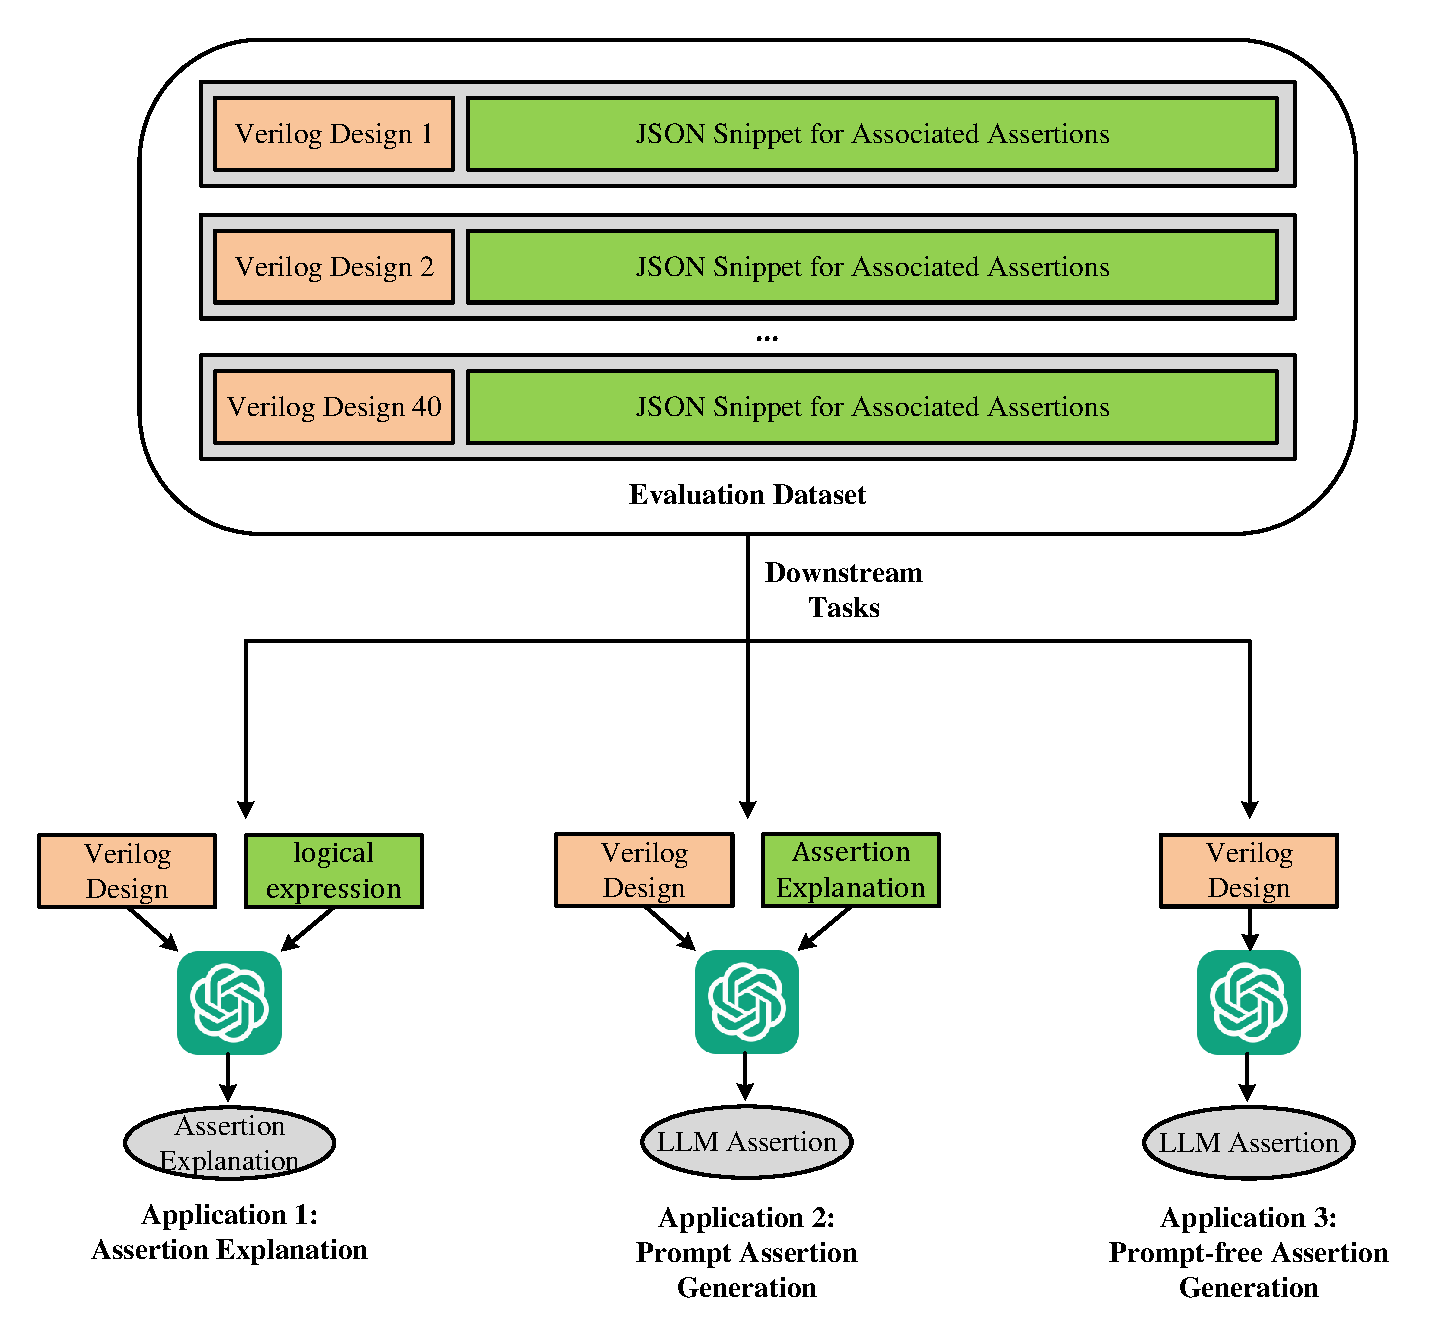
\includegraphics[width=0.8\linewidth]{Figs/Combined_Prompt.pdf}
%     \caption{Combined prompt from RAG framework.}
%     \label{fig:Combined-Prompt}
% \end{figure}

